\documentclass{standalone}
\usepackage{tikz}
\begin{document}
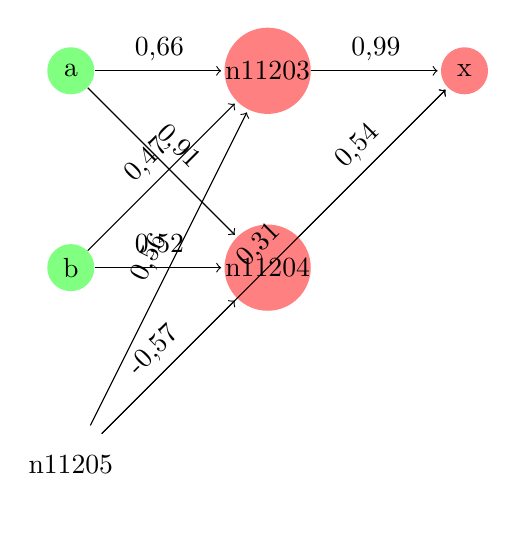
\begin{tikzpicture}[shorten >=1pt,->,draw=black!,node distance=2.5cm]
\tikzstyle{neuron}=[circle,fill=black!25,minimum size=17pt,inner sep=0pt]
\tikzstyle{constant}=[neuron, fill=white!50];
\tikzstyle{identity}=[neuron, fill=green!50];
\tikzstyle{sigmoid}=[neuron, fill=red!50];
\node [identity] (a) {a};
\node [identity,below of=a] (b) {b};
\node [constant,below of=b] (n11205) {n11205};
\node [sigmoid,right of=a] (n11203) {n11203};
\node [sigmoid,below of=n11203] (n11204) {n11204};
\node [sigmoid,right of=n11203] (x) {x};
\path[every node/.style={sloped,anchor=south,auto=false}]
(b) edge node {0,52} (n11204)
(b) edge node {0,47} (n11203)
(n11205) edge node {0,31} (x)
(n11205) edge node {0,56} (n11203)
(n11205) edge node {-0,57} (n11204)
(n11203) edge node {0,99} (x)
(n11204) edge node {0,54} (x)
(a) edge node {0,91} (n11204)
(a) edge node {0,66} (n11203)
;\end{tikzpicture}
\end{document}